\documentclass[8pt]{beamer}

\usetheme{CambridgeUS}
\useinnertheme{rectangles}

\usepackage[utf8]{inputenc}
\usepackage[T1]{fontenc}
\usepackage[ngerman]{babel}
\usepackage[babel,german=quotes]{csquotes}
\usepackage{lmodern}
\usepackage{graphics}
\usepackage{hyperref}
\usepackage{color}
\usepackage{enumerate}
\usepackage{framed}
%\usepackage{pgfpages}
%\pgfpagesuselayout{4 on 1}[a4paper, border shrink=5mm, landscape]
%\pgfpagesuselayout{2 on 1}[a4paper, border shrink=5mm]

\mode<presentation>{
	\hypersetup{pdfpagemode=FullScreen}
}

\setbeamercovered{transparent}
%\beamertemplatenavigationsymbolsempty

\title[]{Bürgerinitiative für eine klima- und gesundheitsschonende Fernwärmeversorgung für Graz }
\subtitle{Günter Eisenhut \& Walter Felber \& Johannes Stigler}
\date[]{}

\begin{document}

	\AtBeginSection[]
	{
  		\begin{frame}
    		\frametitle{Agenda}
    		\tableofcontents[currentsection]
  		\end{frame}
	}
	\frame{\titlepage}
		
	\frame{\frametitle{Agenda}\tableofcontents} 
	
	\section{Was plant die Stadt Graz?}
	\begin{frame}[t]
		\frametitle{Was plant die Stadt Graz?} 
		\begin{itemize}
			\item Geplant ist ein sogenanntes \textquote{Energiewerk}, das eigentlich eine Müllverbrennungsanlage ist.
			\item Im Stadtgebiet von Graz\footnote{Graz hat schon jetzt die schlechtesten Luftwerte, aller Landeshauptstädte} in der Puchstraße sollen jährlich rund 120.000 t Restmüll zum Zwecke der Fernwärmeversorgung verbrannt werden.
			\item Dabei würden mindestens 120.000 t $CO_2$ jährlich entstehen und ein Cocktail aus hochgiftigen, krebserregenden und erbgutschädigende Stoffen wie Quecksilber, Dioxine, Furane etc. in die Umwelt gelangen.
			\item Ein Projekt mit völlig veralteten Technologien und Massenverbrennung wurde schon vor dreißig Jahren erfolgreich von einer Bürgerinititative verhindert. 			
			
			\item Durch das Energiewerk soll Fernwärme für 23.000 Haushalte gewonnen werden. 
			\item Da die Stadt Graz kein Geld hat, soll das Energiewerk durch einen Kredit von über 280.000 Euro finanziert werden, der wieder einmal von den Fernwärmekund:innen über die Fernwärmepreise zurückgezahlt werden müsste.
			
			\item Dadurch würde auch 40 Jahre lang kein Interesse an fortschrittlichen Formen des Recyclings bestehen. Statt die knappen natürlichen Ressourcen optimal zu nutzen, würde möglichst viel verbrannt werden. Und die jetzt schon sehr hohen Fernwärmepreise würden unkontrollierbar weiter steigen.
  		\end{itemize}
	\end{frame}
	


	\begin{frame}[t]
		\frametitle{Graz hat schon jetzt die schlechtesten Luftwerte aller österreichischen Landeshauptstädte} 
		
		Air Quality Index des MSN-Luftgüte Services am 21.1.2024
		\vspace{0.4mm}
		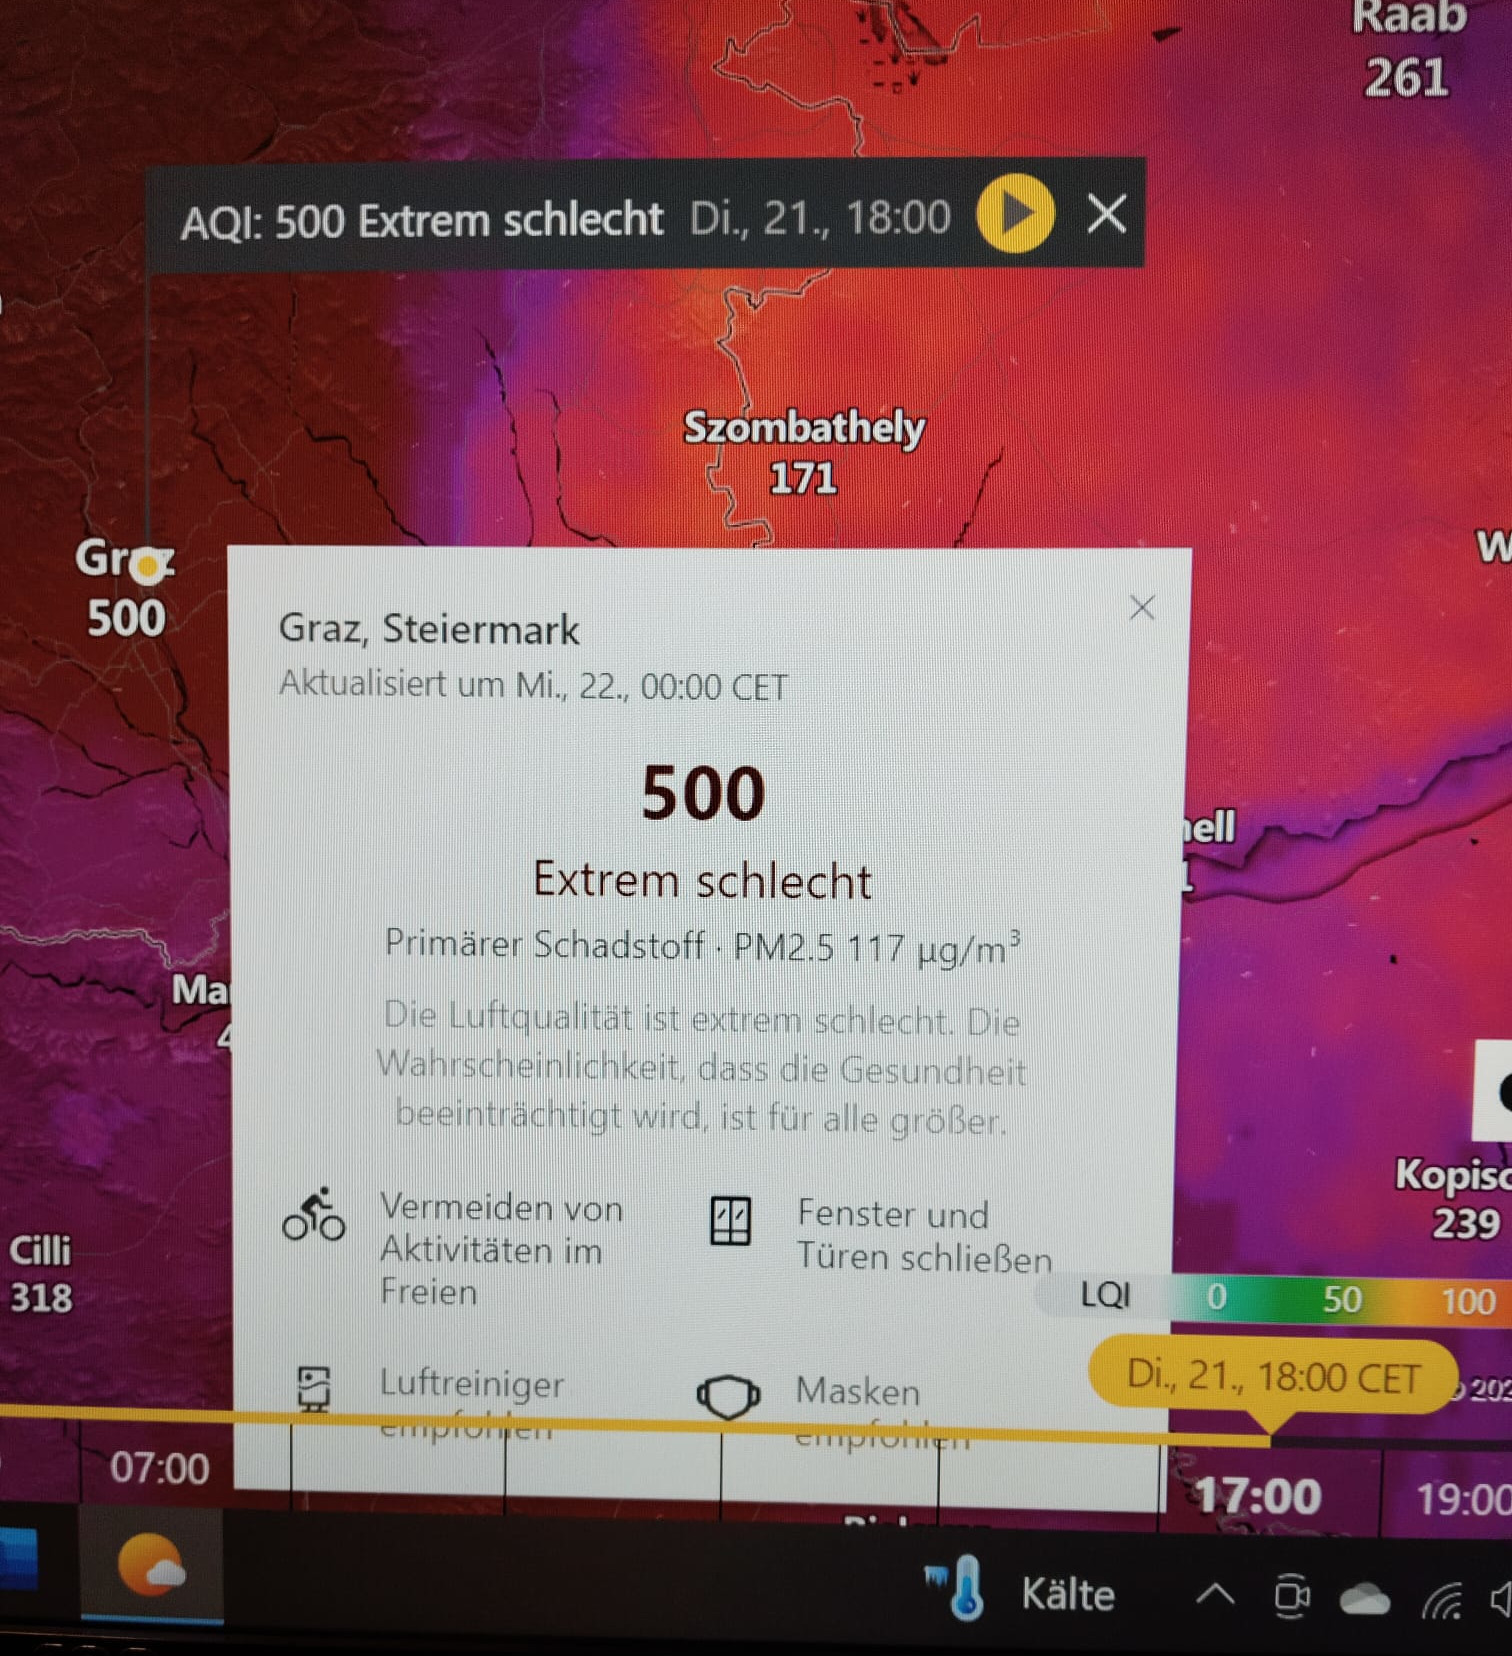
\includegraphics[scale=0.5]{msn.jpg}

	\end{frame}
	
	
	\begin{frame}[t]
		\frametitle{Graz hat schon jetzt die schlechtesten Luftwerte aller österreichischen Landeshauptstädte} 
		
		Luftgütewerte des Luftinformationsdienstes Steiermark ebenfalls am 21.1.2024
		\vspace{0.4mm}
		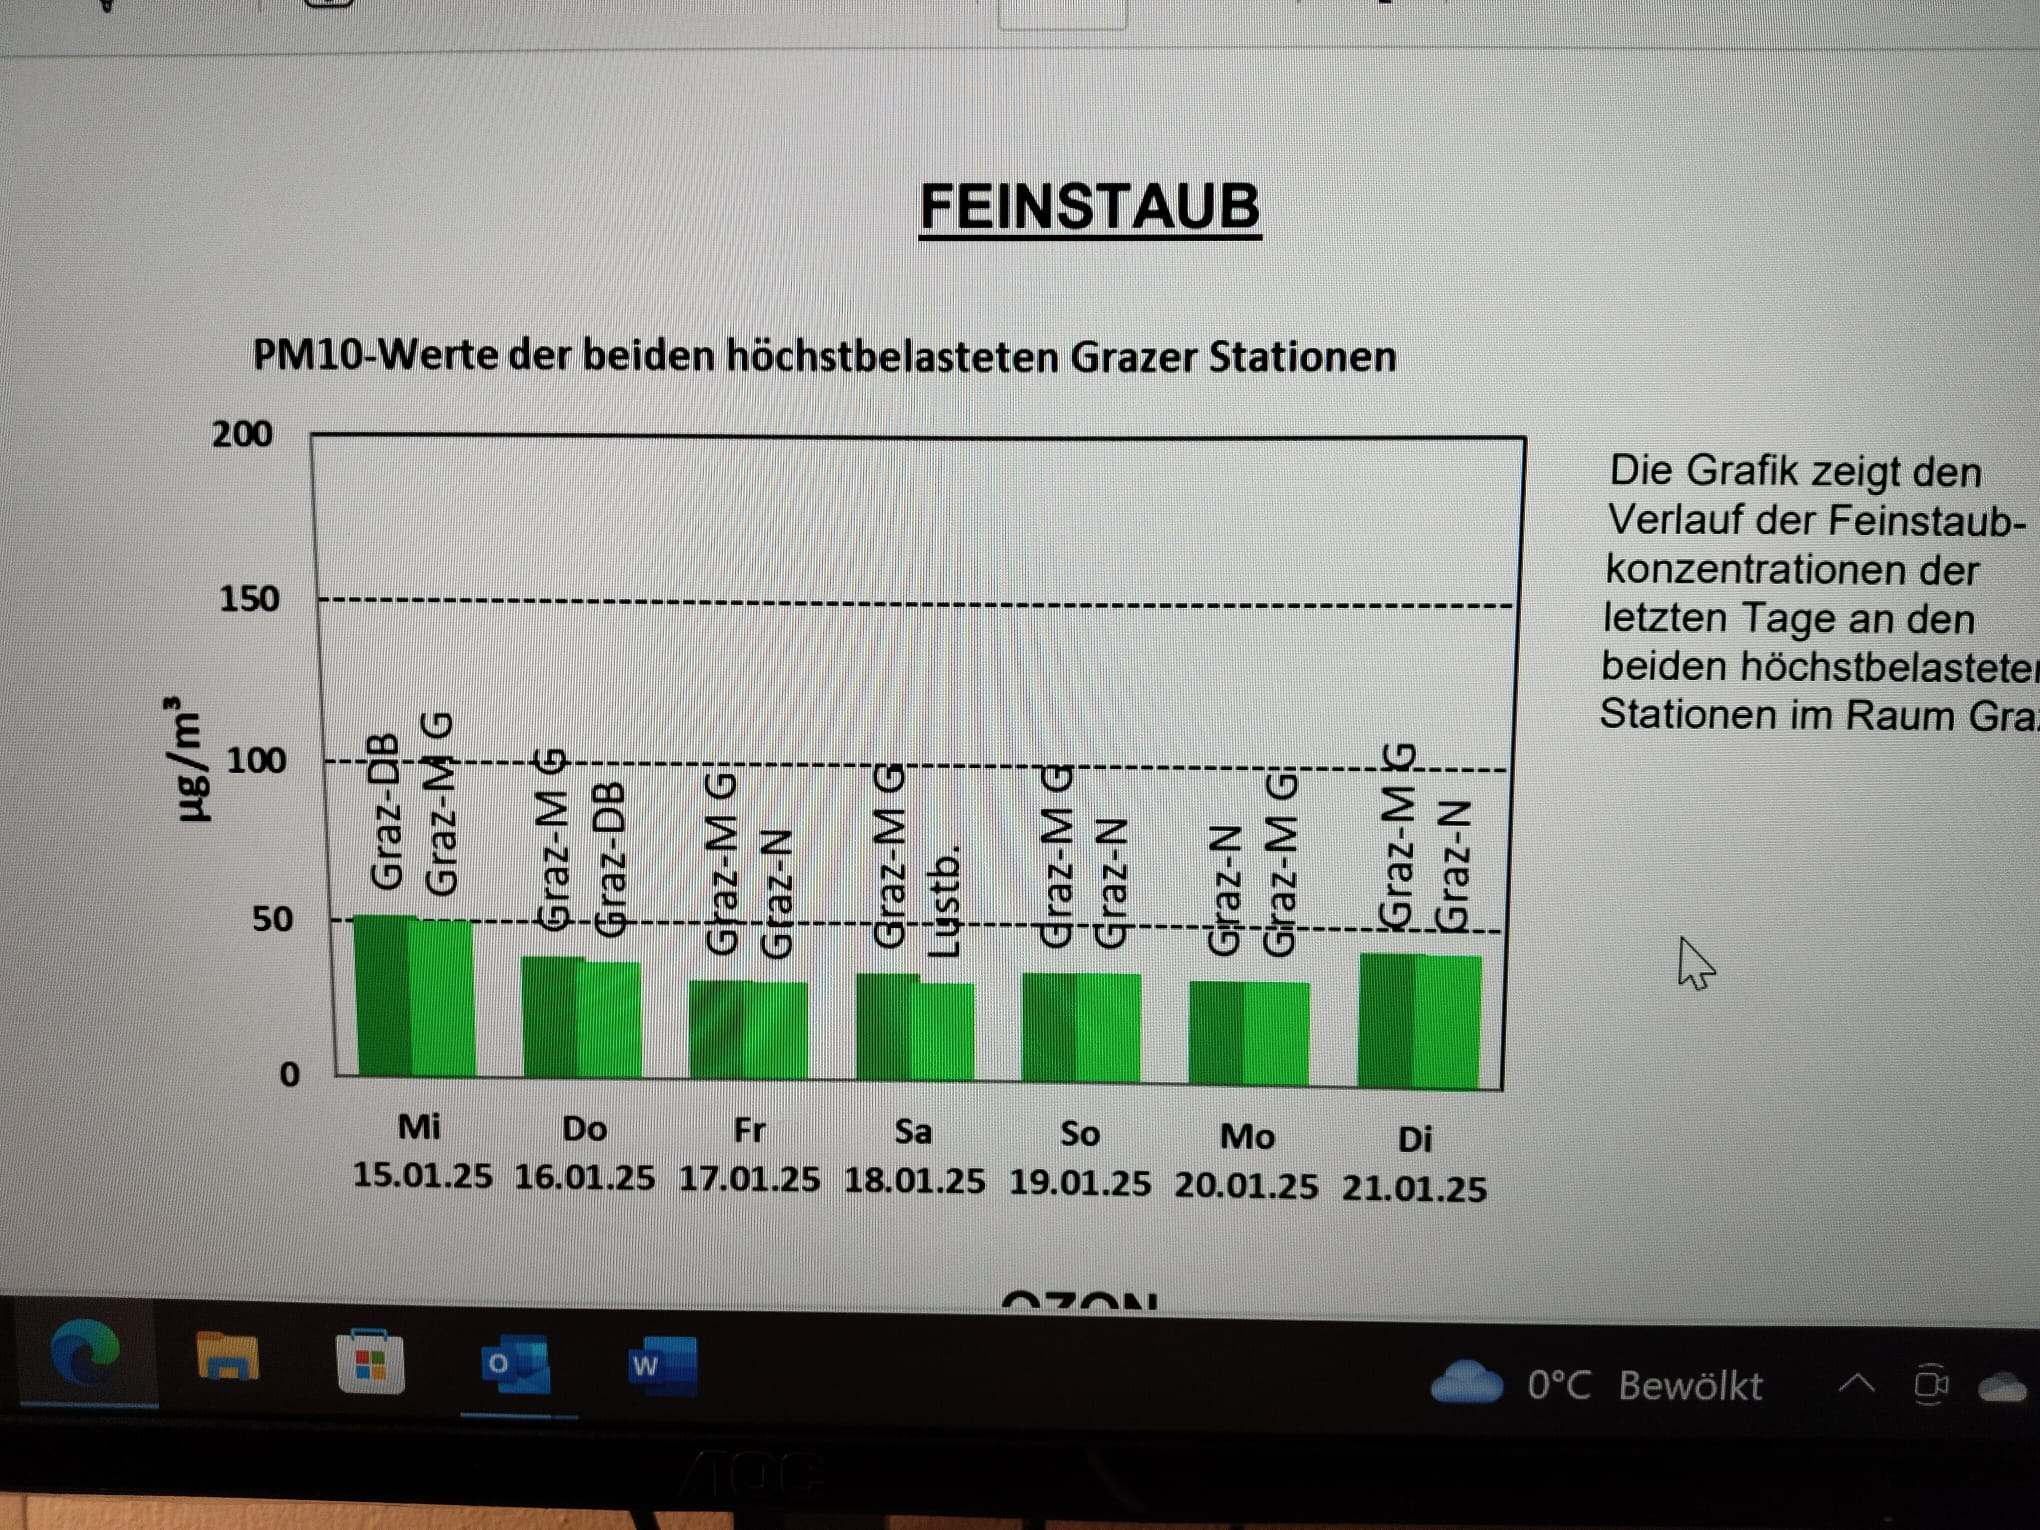
\includegraphics[scale=0.16]{feinstaub.jpg}

	\end{frame}

	\begin{frame}[t]
		\frametitle{Der Kipppunkt ist überschritten: 2023 hat der Wald 5,3 Millionen t $CO_2$ 	emittiert} 
		
		\vspace{0.8mm}
		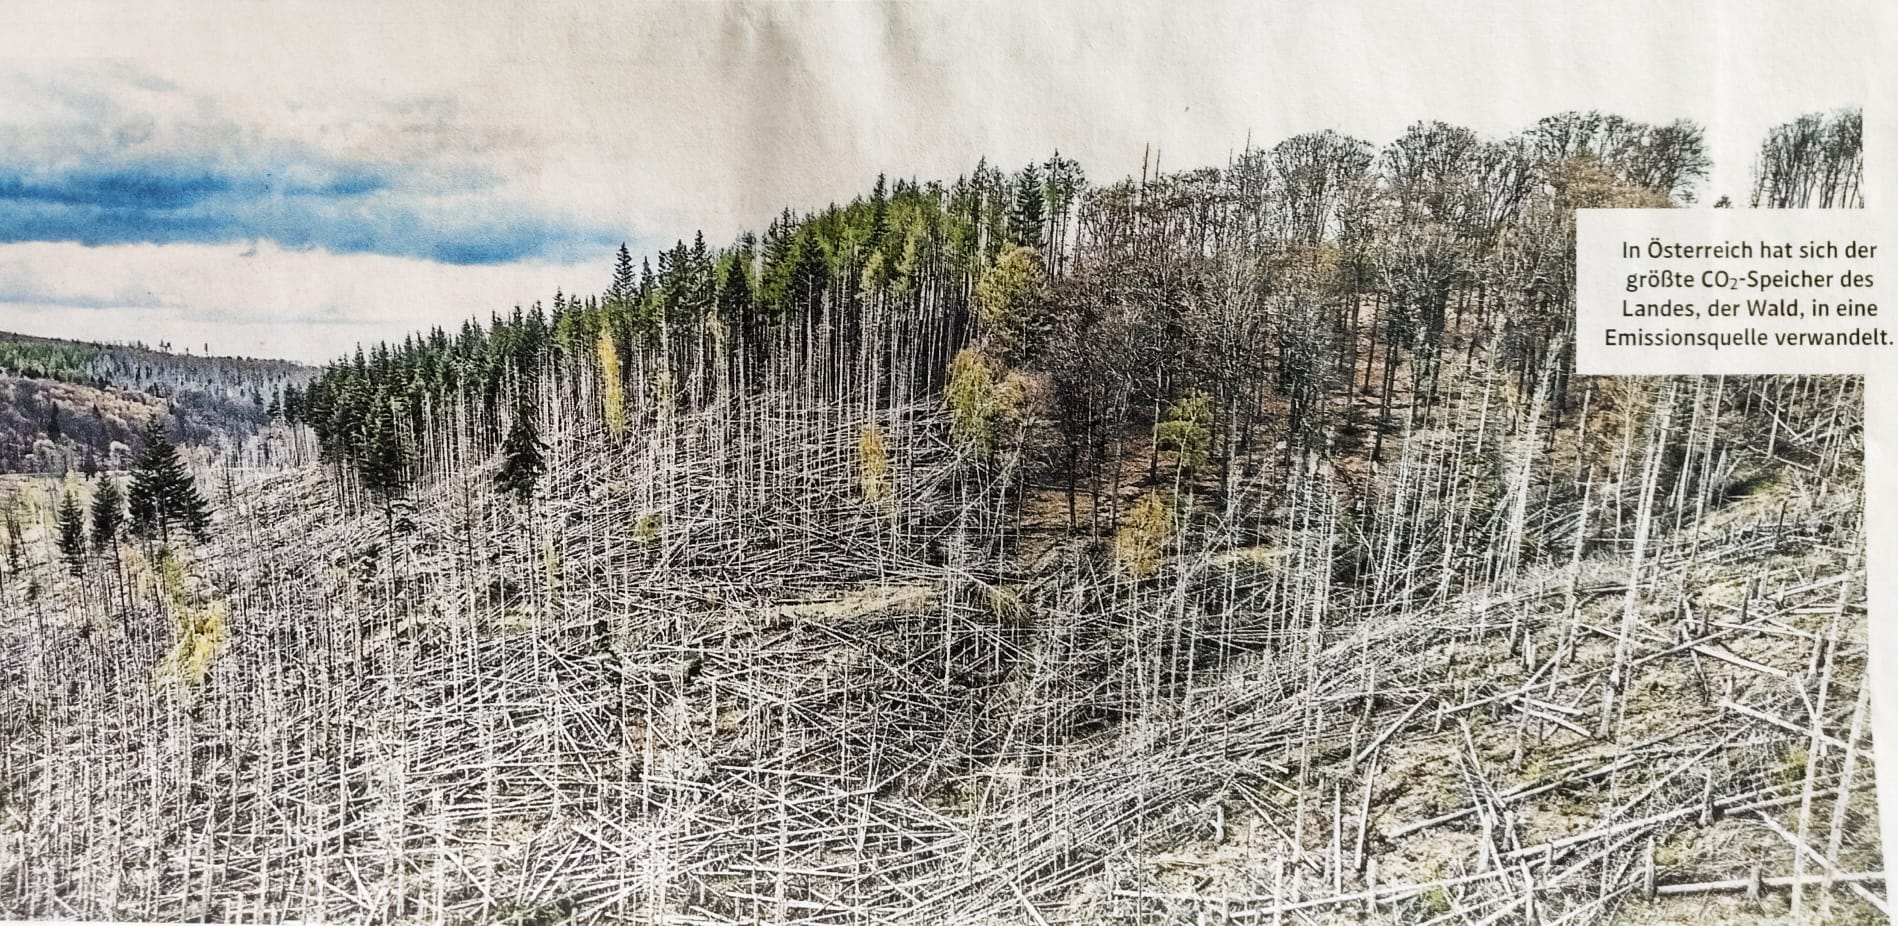
\includegraphics[scale=0.18]{wald.jpg}

	\end{frame}


\section{Eine Gegenüberstellung wichtiger Argumente}

	\begin{frame}[t]
		\frametitle{Eine Gegenüberstellung wichtiger Argumente} 
		\textbf{Nachhaltige Energieversorgung}
		\begin{figure}[htbp]
			\begin{minipage}[t]{0.38\textwidth}
				\textbf{Energie Graz\footnote{Zu finden unter \url{https://www.energie-graz.at/egg/unternehmen/ewg}}}
			\end{minipage}
			\hfill
			\begin{minipage}[t]{0.58\textwidth}
				\textbf{Bürgerinitiative}
			\end{minipage}
		\end{figure}
		\begin{figure}[htbp]
			\begin{minipage}[t]{0.38\textwidth}
				\begin{framed}
				Wir erzeugen 180 GWh ökologische Fernwärme, womit 23.000 Wohnungen versorgt werden können und reduzieren damit das Erdgas in der Fernwärme\-erzeugung und realisieren eine jährlich $CO_2$-Einsparung von 15.000 t.
				\end{framed}
			\end{minipage}
			\hfill
			\begin{minipage}[t]{0.58\textwidth}
				\begin{framed}
				Die Einsparung von 15.000 t wird mit dem Wegfall von Lastwagentransporten
zur Müllverbrennung in die Slowakei begründet. Verschwiegen wird, dass die
Müllverbrennung in Graz 120.000 t $CO_2$ emittiert. So wird die Öffentlichkeit
bewusst getäuscht!
                                  \begin{itemize}
                                        \item Mit Ökologie hat das Vorhaben der Energie Graz rein gar nichts zu tun.
                                                \item Anstelle der 60.000 t Restmüll, die derzeit in Graz und Graz Umgebung anfallen, müssen im Energiewerk rund 120.000 t verbrannt werden, damit das Werk effizient und kostendeckend betrieben werden kann.
                                             \item Und das Verbrennen einer Tonne Restmüll emittiert rund eine Tonne $CO_2$.  
                      \end{itemize}
				\end{framed}
			\end{minipage}
		\end{figure}
	\end{frame}		

	\begin{frame}[t]
		\frametitle{Eine Gegenüberstellung wichtiger Argumente} 
		\textbf{Verkehrsentlastung}
		\begin{figure}[htbp]
			\begin{minipage}[t]{0.38\textwidth}
				\textbf{Energie Graz}
			\end{minipage}
			\hfill
			\begin{minipage}[t]{0.58\textwidth}
				\textbf{Bürgerinitiative}
			\end{minipage}
		\end{figure}
		\begin{figure}[htbp]
			\begin{minipage}[t]{0.38\textwidth}
				\begin{framed}
					Durch die lokale energetische Nutzung der nicht recyclingfähigen Reststoffe werden jährlich 9.000 LKW-Fahrten eingespart. Dadurch reduzieren wir Emissionen, erhöhen die Verkehrssicherheit und steigern die Lebensqualität.				
				\end{framed}
			\end{minipage}
			\hfill
			\begin{minipage}[t]{0.58\textwidth}
				\begin{framed}
				Geht so Verbesserung der Lebensqualität?
                                        \begin{itemize}
                                                \item Geplant ist ein Betrieb der Anlage sieben Tage die Woche und 24-Stunden am Tag.
                                                \item Der zusätzlich benötigte Müll muss mit LKWs angeliefert werden. Unklar bleibt daher was im Betrieb des Energiewerkes wirklich an LKW-Fahrten eingespart werden wird.
                                                \item Unklar bleibt auch wie die jährlich  bei der Verbrennung anfallenden 30.000 t an Aschen und Schlacken abtransportiert werden sollen. Sie sollen \textquote{im Regelfall per Bahn (Schleppbahn)} erfolgen. Was heißt hier \textquote{im Regelfall}?
                                               
                                         
                        \end{itemize}
				\end{framed}
			\end{minipage}
		\end{figure}
	\end{frame}		

	
	\begin{frame}[t]
		\frametitle{Eine Gegenüberstellung wichtiger Argumente} 
		\textbf{Sichere Verwertung}
		\begin{figure}[htbp]
			\begin{minipage}[t]{0.38\textwidth}
				\textbf{Energie Graz}
			\end{minipage}
			\hfill
			\begin{minipage}[t]{0.58\textwidth}
				\textbf{Bürgerinitiative}
			\end{minipage}
		\end{figure}
		\begin{figure}[htbp]
			\begin{minipage}[t]{0.38\textwidth}
				\begin{framed}
				Nicht wiederverwertbare, ungefährliche Reststoffe werden dank lokaler Kreislaufwirtschaft vor Ort energetisch verwertet. Wir sichern damit für 40 Jahre Entsorgungssicherheit für 450.000 Steirer:innen im Großraum von Graz.
			\end{framed}			
			\end{minipage}
			\hfill
			\begin{minipage}[t]{0.58\textwidth}
				\begin{framed}
					Kreislaufwirtschaft geht anders!
					\begin{itemize}
						\item \textquote{Restmüll sind Rohstoffe am falschen Ort}. 
						\item Moderne Recyclingverfahren können bis zum 95\% des bestens aufbereitenden Restmülls einer Wiederverwertung zuführen.
						\item Der Fortschritt bei Recycling und Kreislaufwirtschaft wird blockiert.
					\end{itemize}
				\end{framed}
			\end{minipage}
		\end{figure}		
	\end{frame}		
	
	
		\begin{frame}[t]
		\frametitle{Eine Gegenüberstellung wichtiger Argumente} 
		\textbf{Stabile Preise und neue Arbeitsmärkte}
		\begin{figure}[htbp]
			\begin{minipage}[t]{0.38\textwidth}
				\textbf{Energie Graz}
			\end{minipage}
			\hfill
			\begin{minipage}[t]{0.58\textwidth}
				\textbf{Bürgerinitiative}
			\end{minipage}
		\end{figure}
		\begin{figure}[htbp]
			\begin{minipage}[t]{0.38\textwidth}
				\begin{framed}				
					 Wir werden unabhängiger von internationalen Energie- und Verwertungsmärkten. Das sorgt für Preisstabilität bei den Abfallgebühren und der Fernwärme. Zusätzlich schaffen wir regional 100 neue Arbeitsplätze.
				\end{framed}
			\end{minipage}
			\hfill
			\begin{minipage}[t]{0.58\textwidth}
				\begin{framed}
				Insgesamt wird das Projekt die Preise für die Fernwärme hochhalten.
                \begin{itemize}
                  \item Weil das Energiewerk über Kredite finanziert wird und zusätzlich auch  Abhängigkeiten vom Kapitalmarkt entstehen.
                  \item Weil zusätzlich Kosten für $CO_2$-Zertifikate anfallen.
                  \item Weil es keine Förderungen für diese veraltete Technologie gibt. 
                  \item Weil die Baukosten bis zu dreimal höher als bei modernen, emissionsarmen Technologien sind.
                  \item Außerdem schafft ein sinnvolles Recycling mindestens ebensoviele und noch dazu ökologisch sinnvolle Arbeitsplätze.
                 \end{itemize}
				\end{framed}
			\end{minipage}
		\end{figure}
	\end{frame}		
	
 \begin{frame}[t]
		\frametitle{Eine Gegenüberstellung wichtiger Argumente}
		\textbf{Investition in die Zukunft} 
		\begin{figure}[htbp]
			\begin{minipage}[t]{0.38\textwidth}
				\textbf{Energie Graz}
			\end{minipage}
			\hfill
			\begin{minipage}[t]{0.58\textwidth}
				\textbf{Bürgerinitiative}
			\end{minipage}
		\end{figure}
		\begin{figure}[htbp]
			\begin{minipage}[t]{0.38\textwidth}
				\begin{framed}				
				Wir investieren auf dem Industriegelände am Standort Puchstraße, direkt angrenzend an die Abfallbehandlungsanlage der Holding Graz, in eine nachhaltige Zukunft. Mit modernster Kraft-Wärme-Kopplung und Integration von hocheffizienten Wärmepumpensystemen produzieren wir ganzjährig Wärme und Strom. Die beste verfügbare Technik kommt zum Einsatz und sichert Effizienz und Umweltschutz.
				\end{framed}
			\end{minipage}
			\hfill
			\begin{minipage}[t]{0.58\textwidth}
				\begin{framed}
                \begin{itemize}
                  \item Ja, wenn das wirklich so ist, warum dann noch Müllverbrennung? Großwärmepumpen sind heute problemlos in der Lage die benötigten 180 GWh zu liefern und das noch viel kostengünstiger (z.B. Helsinki oder Köln).
                  \item Die geplante Technik des Energiewerk ist veraltet und entspricht weder im Bereich der thermischen Müllentsorgung (Rostfeuerung versus Wirbelschichtverfahren) noch im Bereich der Wärmeerzeugung dem aktuellen verfahrenstechnischen Stand.
                 \end{itemize}
				\end{framed}
			\end{minipage}	
			\end{figure}
\end{frame}			
			
	\section{Zentrale Argumente der Bürgerinitiative}
	\begin{frame}[t]
		\frametitle{Zentrale Argumente der Bürgerinitiative} 
		\begin{itemize}
			\item Das geplante Energiewerk in Graz ist eine Energiewende in die falsche Richtung, in die fossile Vergangenheit statt in die emissionsfreie Zukunft. 
			\item Riesige Mengen von Plastik und Kohlenstoff im Müll würden verbrannt anstatt einer Wiederverwertung zugeführt werden. 		
			\item Das würde den Klimazielen widersprechen und die Stadt Graz will bis 2040 klimaneutral sein.
			\item Und es gibt bereits heute neue, bessere und kostengünstigere Lösungen für eine Fernwärme­versorgung: Abwärmenutzung, Tiefenwärme, Großwärmepumpen, Solarthermie u.a.
			\item Aber auch bessere und kostengünstigere Lösungen für eine sinnvolle Aufbereitung des Restmülls, über die große Teile des Mülls einer Wiederverwertung zugeführt werden können. 
			\item \textquote{Restmüll sind Rohstoffe am falschen Ort}, wie einschlägige Expert:innen formulieren. 			
  		\end{itemize}
	\end{frame}
	
	
	\section{Weitere Vorgehensweise}
	\begin{frame}[t]
		\frametitle{Weitere Vorgehensweise} 
		\begin{itemize}
			\item Es gilt bis 24. Mai 200 Unterstützungsunterschriften zu sammeln
		    \item Damit die Bürgerinitiative im Rahmen der Umweltverträglichkeitsprüfung (UVP) ihre Bedenken gegen das Projekt einbringen kann und verlangen kann, dass es von Amtsgutachtern im Rahmen der UVP genau auf ihre Auswirkungen auf Gesundheit- und Klimaziele überprüft wird.
  		\end{itemize}
	\end{frame}

\end{document}